\subsection{Event Monitoring}

Sometimes it can be useful to monitor the actions Dimple takes as the model or data changes or as inference is performed. Such monitoring can be helpful when debugging your model, when trying to determine whether inference has converged while using belief propogation on a loopy graph, or when attempting to determine whether a graph has been adequately mixed when using the Gibbs solver. To address this need, Dimple provides an event-based system consisting of events that can be triggered when various actions of interest occur and associated event handlers and an event listener that handles dispatching of events. The event system is designed to have no effect on the performance of inference when it has not been enabled, but may have a noticeable effect when it is being used.

The full power of the event system is only available directly in the Java API but the MATLAB API does provide a simple event logging interface that allows events to be logged to the console or an external log file.

\subsubsection{Event types}

\begin{figure}[H]
  \centering
  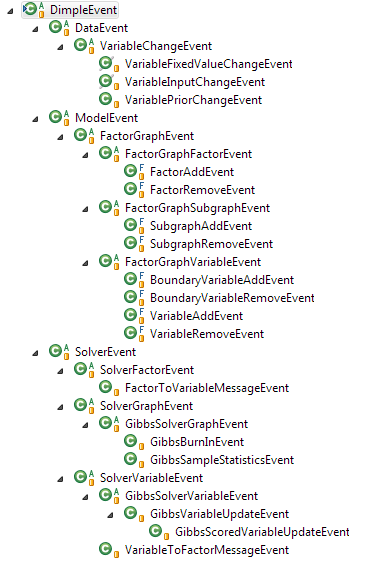
\includegraphics{images/EventHierarchy.png}
  \caption{Dimple event hierarchy}
  \label{fig:EventHierarchy}
\end{figure}

Dimple Events are organized hierarchically, and the current version of the full hierarchy is shown in Figure \ref{fig:EventHierarchy}. Note that any event types marked with an 'A' in the diagram are abstract super types and are used to organize the events by category. Actual event instances will belong to non-abstract types, which are for the most part leaf-nodes in the diagram. Events are subdivided into three categories:

\begin{itemize}
\item ModelEvent: includes changes to the structure of the model including adding and removing variables, factors and subgraphs. The concrete model event types are:
  \begin{itemize}
  \item FactorAddEvent and FactorRemoveEvent: raised when a factor is added or removed from the model.
  \item VariableAddEvent and VariableRemoveEvent: raised when a variable is added or removed from the model.
  \item SubgraphAddEvent and SubgraphRemoveEven: raised when a subgraph is added or removed from the model.
  \item BoundaryVariableAddEvent and BoundaryVariableRemoveEvent: raised when a boundary variable is added or removed.
  \end{itemize}
\item DataEvent: includes changes to data including changes to fixed values and inputs. The concrete data event types are:
  \begin{itemize}
  \item VariablePriorChangeEvent: raised when a prior is changed on a variable.
  \item VariableFixedValueChangeEvent (deprecated): raised when a fixed value prior is set or unset on a variable. This event type has been subsumed by VariablePriorChangeEvent and will eventually be discontinued.
  \item VariableInputChangeEvent (deprecated): raised when a prior distribution is set or unset on a variable. This event type has been subsumed by VariablePriorChangeEvent and will eventually be discontinued.
  \end{itemize}
\item SolverEvent: includes solver-specific events of interest that occur while running inference. The concrete event types are:
  \begin{itemize}
  \item FactorToVariableMessageEvent and VariableToFactorMessageEvent: raised when edge messages are updated in belief propagation solvers. Currently only the sumproduct and minsum solvers generate these messages.
  \item GibbsBurnInEvent: raised upon completion of random-restart and burn-in phase of Gibbs solver.
  \item GibbsSampleStatisticsEvent: raised after generation of one set of samples for the graph have been generated by the Gibbs solver. Contains statistics relevant to the sample.
  \item GibbsVariableUpdateEvent and GibbsScoredVariableUpdateEvent: raised when sample values are changed by the Gibbs solver. The two event types are the same except that the scored version adds information about the change in score induced by the sample update.
  \end{itemize}
\end{itemize}

Additional events may be added in future releases. New event types may also be added by developers who have extended Dimple with their own solvers or custom factors in Java.

\ifmatlab
When specifying event types in the MATLAB API, use the event type name in a string value:

\begin{figure}[H]
\begin{lstlisting}
logger = getEventLogger();
logger.log('FactorToVariableMessageEvent', fg);
\end{lstlisting}
\end{figure}

Unrecognized event types will result in an exception.

Note that Dimple events are not MATLAB events and you cannot use MATLAB's event API to trigger or listen for Dimple events.
\fi

\ifjava
When specifying event types in the Java API, use the event class itself:

\begin{figure}[H]
\begin{lstlisting}
DimpleEventLogger logger = new DimpleEventLogger();
logger.log(FactorToVariableMessageEvent.class, fg);
\end{lstlisting}
\end{figure}
\fi

\FloatBarrier

\subsubsection{Event logging}

The easiest way to monitor events in Dimple is through an event logger. Given an event logger instance, you can configure it to log either to the console or to a text file, you can configure how verbose the output should be, and specify which events for which model objects should be logged.

\ifmatlab
Event loggers are instances of the EventLogger class. You may create an
instance using the constructor:

\begin{figure}[H]
\begin{lstlisting}
logger = EventLogger();
\end{lstlisting}
\end{figure}

or you may simply get the default global instance using the getEventLogger() function, which will create a new logger the first time it is invoked:

\begin{figure}[H]
\begin{lstlisting}
logger = getEventLogger();
\end{lstlisting}
\end{figure}
\fi

\ifjava
Event loggers are instances of the DimpleEventLogger class. You may create a new one using the constructor:

\begin{lstlisting}
DimpleEventLogger logger = new DimpleEventLogger();
\end{lstlisting}
\fi

Newly constructed loggers will output to standard error by default and will have a default verbosity of zero, which will produce the most terse output. You may configure the logger to change the verbosity level or to direct output to a different target. For example:

\begin{figure}[H]
\ifmatlab
\begin{lstlisting}
% Use more verbose log output.
logger.Verbosity = 2;

% Append output to a file in the working directory.
logger.open('event-logger.txt');

% ... or output to standard output
logger.open('stdout');
\end{lstlisting}
\fi

\ifjava
\begin{lstlisting}
// Use more verbose log output.
logger.verbosity(2);

// Append output to a file in the working directory.
logger.open(new File("event-logger.txt"));

// ... or output to standard output
logger.open(System.out);
\end{lstlisting}
\fi
\end{figure}

Usually a single logger will be sufficient, but you can create multiple logger objects that direct output to different targets.

To enable logging for a particular class of events on your model, use the log method with the event type of interest. If the event type is abstract (is annotated with the letter A in Figure \ref{fig:EventHierarchy}), then
all event subtypes will be logged. If the event type is not abstract, then
only that particular event type will be logged. In particular, if you specify SolverEvent on a graph using the Gibbs solver, you will see
GibbsScoredVariableUpdateEvent messages but if you specify
GibbsVariableUpdateEvent you will get only messages for that specific
class and will not get scored messages.

\begin{figure}[H]
\ifmatlab
\begin{lstlisting}
% Log all solver events for given model.
logger.log('SolverEvent', model);

% Log unscored Gibbs update messages
logger.log('GibbsVariableUpdateEvent', model);

% Log variable to factor messages for a single variable
logger.log('VariableToFactorMessageEvent', x);
\end{lstlisting}
\fi

\ifjava
\begin{lstlisting}
// Log all solver events for given model.
logger.log(SolverEvent.class, model);

// Log unscored Gibbs update messages
logger.log(GibbsVariableUpdateEvent.class, model);

// Log variable to factor messages for a single variable
logger.log(VariableToFactorMessageEvent.class, x);
\end{lstlisting}
\fi
\end{figure}

You may remove previously created log registration either by
using the unlog method to remove individual entries or the clear
method to remove all entries. When using unlog, the arguments must
match the original arguments passed to log. (Note that setting the verbosity to a negative value or closing the output will also turn off logging it will not prevent Dimple from creating the underlying events, so make sure to use the clear() method when you are done with logging if you do not want to slow down inference.)

\begin{figure}[H]
\ifmatlab
\begin{lstlisting}
% Disable a previous log registration
logger.log('SolverEvent', model);

% Disable all logging
logger.clear();
\end{lstlisting}
\fi

\ifjava
\begin{lstlisting}
// Disable a previous log registration
logger.log(SolverEvent.class, model);

// Disable all logging
logger.clear();
\end{lstlisting}
\fi
\end{figure}

When using logging, it is usually very helpful to give the variables, factors and
subgraphs unique, easy to read, names. This will make your log output much easier to understand.

\subsubsection{Advanced event handling}

\ifmatlab
The MATLAB API does not support handling Dimple events outside of the EventLogger
class. More advanced uses cases may be implemented using the Java API. See the Java version of this manual for details.
\fi

\ifjava
The DimpleEventLogger class provides an easy way to monitor changes when
running inference in Dimple, but it does not let you interact directly with 
the event objects or take actions other than simple logging. A much wider range of
options is available by using the event handler and listener framework upon which the
logger is based. This is described in more detail in the next sections.

\subsubsection{Event listeners}
An object of type DimpleEventListener may be attached to the root FactorGraph of the model by the FactorGraph.setEventListener method and will be used to dispatch all events generated by the model and its associated data and solver layers. If there is no listener on the root graph, then no events should be generated. By default there is no listener for newly created graphs. When creating a listener, you can either create a new instance or use the global default instance that is lazily created by DimpleEventListener.getDefault(). Note that the DimpleEventLogger automatically adds the default listener to the root graph of models that don't already have a listener when a new log specification is registered for a child of the graph, but you will need to do this explicitly if you are not using that class.

Once a listener has been associated with the graph, then one or more handlers may be registered to handle events on the graph. The registration must specify the base class of the type of event to be handled and the root object on which events will be raised. It will be easiest to register for events at the root graph, but it may sometimes be desirable to set up handlers for specific variables, factors or subgraphs. For instance, to register handlers for various belief propagation messages on a graph, you could write: 

\begin{figure}[H]
\begin{lstlisting}
DimpleEventListener listener = DimpleEventListener.getDefault();
fg.setEventListener(listener);
listener.register(factorMessageHandler,
    FactorToVariableMessageEvent.class, fg);
listener.register(variableMessageHandler,
    VariableToFactorMessageEvent.class, fg);
\end{lstlisting}
\end{figure}

Handlers can be removed by one of the various unregister methods on the listener; see the Java API doc for that class for details. Changes to event registration or the value of the root listener are not guaranteed to take effect until the next time the affected objects have been initialized or the IDimpleEventSource.notifyListenerChanged() method has been invoked on the object that generates the event. This is important for model events in particular since model changes typically occur prior to initialization. 

\subsubsection{Event handlers}
Dimple event handlers are objects that implement the IDimpleEventHandler interface. In practice most handlers should simply extend the abstract base class DimpleEventHandler. For example, here is a simple handler class that simply prints events out to the console with a verbosity of one: 

\begin{figure}[H]
\begin{lstlisting}
public class EventPrinter extends DimpleEventHandler<DimpleEvent>
{
    public void handleEvent(DimpleEvent event)
    {
        event.println(System.out, 1);
    }
}
\end{lstlisting}
\end{figure}

Handler classes that are specific to a particular event subclass can be parameterized appropriately to avoid the need for downcasts. For example, here is a simple handler that keeps a running total of the total graph score during Gibbs sampling based on sample score differences:

\begin{figure}[H] 
\begin{lstlisting}
public class RunningScoreHandler extends DimpleEventHandler<GibbsScoredVariableUpdateEvent>
{
    public double score;

    RunningScoreHandler(double startingScore)
    {
        score = startingScore;
    }

    public void handleEvent(GibbsScoredVariableUpdateEvent event)
    {
        score += event.getScoreDifference();
    }
}
\end{lstlisting}
\end{figure}

\fi